\begin{center}
    \vspace{5cm}
    {\Huge\textbf{\section{\underline{Decisions}}}} % Large and bold text
    \begin{figure}[h]
        \centering
        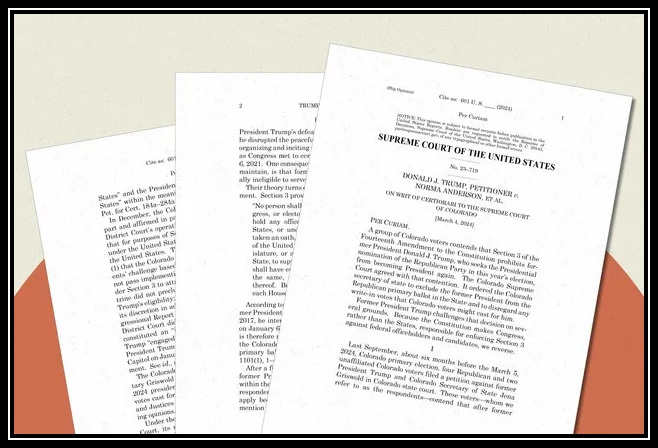
\includegraphics[width=0.7\textwidth]{Figures/intro_page_images/decision_image_1.jpg} \\
        \footnotesize{Photo Credit: POLITICO Illustration (Politico)} \\
        \vspace{2mm}
        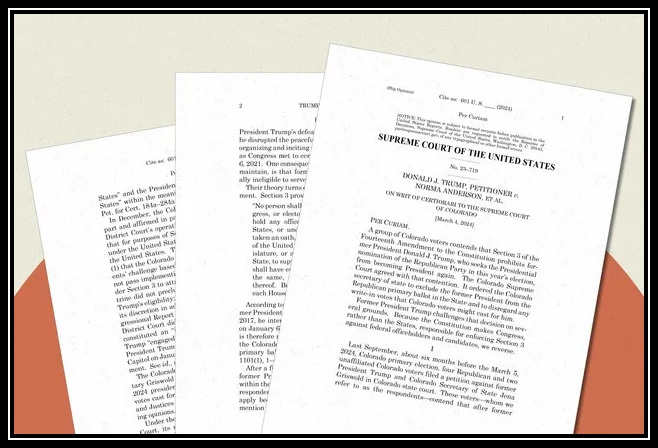
\includegraphics[width=0.7\textwidth]{Figures/intro_page_images/decision_image_1.jpg} \\
        \footnotesize{Photo Credit: Courtroom sketch by Bill Hennessy (CNN)} \\

    \end{figure}
\end{center}

\newpage

\begin{center}

\begin{table}[H]
    \centering
    \caption{What's Included (Decisions)}
    \label{tab:example}
    \vspace{1mm}
    \begin{tabularx}{\textwidth}{>{\centering\arraybackslash}p{0.33\textwidth}>{\centering\arraybackslash}X}
        \toprule
        Topic & Description \\
        \midrule
        Justice Agreement Matrix & \RaggedRight Percentage of decisions where Justices coalesced similarity -- i.e., were \emph{both} in Majority or Dissent (ex: Justices Alito and Sotomayor) \\
        \addlinespace
        Decision Overviews & \RaggedRight 2023 Term Decisions organized by sitting (month) with corresponding summary of case-level issue, docket number, holding, opinion author, and coalition size. \\
        \addlinespace
        Decisions by Coalition and Term & \RaggedRight Summary of decisions by coalition size between 2018 and 2023 Terms. \\
        \addlinespace
        Share of Cases Decided (9-0) by Term & \RaggedRight Percentage of cases decided (9-0) between 2018 and 2023 Terms. \\
        \addlinespace
        Share of Cases with Filed Dissent or Concurrence by Term & \RaggedRight Percentage of cases where a dissent or concurrence were filed between 2018 and 2023 Terms. \\
        \addlinespace
        Opinion Lengths & \RaggedRight Top-10 Longest and Shortest Opinions of 2023 Term, well as average opinion lengths by decision type \\
        \addlinespace
        Decision Turnover & \RaggedRight Average number of days elapsed between oral arguments \& decision by the Court (organized by argument sitting and term).\\
        \addlinespace
        Frequency in Majority by Term & \RaggedRight Percentage of cases where each Justice was in the majority between 2018 and 2023 Terms \\
        \addlinespace
        Frequency of Opinion Authorship by Justice and Term & \RaggedRight Percentage of cases where each Justice was the majority opinion author between 2018 and 2023 Terms. \\
        \bottomrule
    \end{tabularx}
\end{table}
\end{center}

\newpage

\begin{center}
\vspace{5mm}
\Huge\textbf{\subsection{\underline{Note on Decision Coding}}}
\end{center}

\noindent We recognize that the array of potential case-level votes do not always neatly align with a definitive indicator that a Justice should be considered a member of the Majority or Minority (\emph{Dissenting}) coalition. In particular, votes by Justices concurring and dissenting \emph{In Part}, \emph{Concurring in Judgement}, joining (and/or authoring) several concurrences, etc., are not as clear of an indicator as authoring or simply joining the majority. These special votes could lead to varying records of majority and minority coalitions sizes depending on the source. For example, a decision rendered with a single Justice authoring an opinion \emph{Concurring In Part, and Dissenting in Part} could reasonbly be coded as either (9-0) or (8-1), given that the Justice neither fully joined -- nor fully dissented -- from the Court's majority opinion. \\

To maintain methodological consistency, we code choices to join the \textbf{Minority} as instances where a Justice (1) Authored a Dissenting Opinion or (2) \textbf{Only} Joined a Dissenting Opinion. Below we list the cases impacted by this coding scheme. \\

\begin{itemize}

\item \emph{Acheson Hotels LLC v. Laufer} (22-429) -- Decided 12/05/2023
\item \emph{Trump v. Anderson} (23-719) -- Decided 03/04/2024
\item \emph{Muldrow v. City of St. Louis} (22-193) -- Decided 04/17/2024
\item \emph{Vidal v. Ester} (23-704) -- Decided 06/13/2024
\item \emph{Starbucks Corp. v. McKinney} (23-367) -- Decided 06/13/2023

\end{itemize}


